\documentclass{article}
\usepackage[english]{babel}
\usepackage[letterpaper,top=2cm,bottom=2cm,left=3cm,right=3cm,marginparwidth=1.75cm]{geometry}
\usepackage{enumitem}
\usepackage{amsmath}
\usepackage[colorlinks=true, allcolors=blue]{hyperref}
\usepackage{minted}
\usepackage{float}
\usepackage{graphicx}
\usepackage{multirow}
\usepackage{subcaption}
\usepackage{booktabs}
\usepackage[utf8]{inputenc}
\usepackage{textgreek}
\usepackage[toc,page]{appendix}
\usepackage{xcolor}
\usepackage{nameref}
\usepackage{url}
\usepackage[T1]{fontenc}
\usepackage{todonotes}
\title{Assignment 4}
\author{Aaron Bussche \and  David Magaram\\[0.3em] Group 28 \and Jason Kasdiran}
\begin{document}
	\maketitle

\listoftodos
\todo[inline]{GLOBAL: target grade 8+. Rubric-driven checklist below. Remove todos before submit.}


\section*{Introduction}
Evolutionary algorithms (EA) are a population-based optimization method. They are based on natural selection and work by exploring new solution areas and iteratively refining good already found solutions, where candidate solutions are improved by mutating and crossover. A common issue is the trade-off between exploration and exploitation. Too much exploration can lead to slow convergence, while too much exploitation can cause suboptimal solutions. Despite this, EAs are still very useful, especially for larger, more complex problems. However, their performance depends on parameter configurations such as mutation rate, population size, and selection pressure.

By investigating the traveling salesman problem and string search, this project explores how different parameter configurations influence convergence speed, population diversity, and algorithm performance. It also aims to explore how mutation rate and selection pressure shape the exploration-exploitation trade-off in these settings, and whether a 2-opt local search can outperform a standard EA algorithm on the traveling salesman problem under fair settings.




\section*{Methods}
This project will implement a genetic algorithm (GA) for string search and memetic algorithm (MA) for traveling salesman problem. This section describes the experimental setup and design choices.
All algorithms were run single-threaded on a desktop system with a AMD Ryzen 5800x processor.
\subsection*{String search}
A string search genetic algorithm was implemented and the used parameters are displayed in Table 1. "NaturalComputing" was used as the target string with a length L = 16, containing both lowercase and uppercase letters from an alphabet $|\Sigma|$. Since fitness is the number of characters that match the target, the maximum fitness is 16. 

The algorithm aims to match the target string by evolving a population of N = 200 individuals. 
Each generation follows a few simple steps. First, during the tournament selection phase, a random subset K is drawn from the population N and the fittest string is kept for reproduction. 

Larger K values mean more potentially high-fitness strings, which can lead to the selection of only the best performers, working as a filter against weaker candidates. While it usually leads to faster convergence, it can also reduce diversity as the entire population will mimic the strongest strings. 

Then, each pair undergoes single-point crossover with a probability $p_c$ = 1, producing 2 new offsprings. Crossover selects a random index and swaps the parent's characters beyond that cutoff. Additionally, every character of the offspring has a small mutation rate $\mu$ to randomly become one of the letters from the alphabet $|\Sigma|$.
Finally, the entire parent generation is replaced with the new offspring generation.

Population diversity was measured using the mean pairwise Hamming distance computed on a random subsample of the population and the average position-wise Shannon entropy \[H_i = -\sum_j f_{ij} \log f_{ij},\] where $f_{ij}$ is the frequency of character j at position i. 
Furthermore, run is terminated if it reaches target string or the maximum generations $G_{max}$ = 200. In case the target is not reached, run is recorded as $t_{finish}$ = $G_{max}$.


\begin{table}[h]
\centering
\caption{String Search GA Parameters}
\begin{tabular}{ll}
\hline
\textbf{Parameter} & \textbf{Value} \\
\hline
String length $L$ & 16 \\ %NaturalComputing
Alphabet $|\Sigma|$ & 52 \\
Population size $N$ & 200 \\
Tournament selection $K$ & $\{2, 5\}$ \\
Crossover probability $p_c$ & 1 \\
Mutation rate $\mu$ & $\{0,\; 1/L,\; 3/L\}$ + sweep from 0/L to 10/L \\
Runs & 10 \\
Max generations $G_{\max}$ & 200 \\
\hline
\end{tabular}
\caption{Parameters for Exercise B1.}
\end{table}


\subsection*{Traveling Salesman Problem}
For the TSP, both a simple evolutionary algorithm (EA) and a memetic algorithm (MA) were implemented. Each solution is encoded as a permutation of city indices representing a tour. The simple EA uses ordered crossover (OX): a random contiguous segment is copied from one parent and the remaining cities are filled in the order they appear in the second parent. Mutation is applied via swap mutation, where two randomly selected positions in the tour are exchanged. Tournament selection ($K = 5$) is used to select parents, and generational replacement with no elitism is applied.

The memetic algorithm extends the EA by applying 2-opt local search to each individual after mutation. The 2-opt procedure iteratively reverses sub-sequences of the tour to eliminate crossing edges, repeating until no improving swap can be found. This Lamarckian approach allows individuals to locally optimize their fitness before evaluation, which typically accelerates convergence. Both algorithms were evaluated on the TSPLIB benchmark instance \textit{eil51} and on the 50-city dataset from the Symmetric Traveling Salesman Problem benchmark instances available at http://comopt.ifi.uni-heidelberg.de/software/TSPLIB95/.

Table 3 displays the used parameters. These parameters were chosen based on the previous exercise and further adjusted based on testing. The crossover probability was lowered to 0.8. This is high enough to help produce new better solutions, but not too high as to break already good solutions. Moreover, mutation was set to 0.3 to explore the area around solutions, and tournament selection was set to 5 as it accelerates convergence and works fairly well. Overall, these parameter settings provide balance between exploration and exploitation. 

\begin{table}[h]
\centering
\begin{tabular}{ll}
\hline
\textbf{Parameter} & \textbf{Value} \\
\hline
Population size $N$ & 100 \\
Tournament selection $K$ & 5 \\
Crossover probability $p_c$ & 0.8 \\
Mutation rate $\mu$ & 0.3 \\
Local search & 2-opt \\
Runs & 10 \\
Max generations $G_{\max}$ & 200 \\
Datasets & eil51 (TSPLIB), 50-city instance\\
Stopping criterion & Fixed generations / wall-clock budget \\
2-opt termination & Until no improving 2-swap remains \\
\hline
\end{tabular}
\caption{Parameters for Exercise B2.}
\end{table}



\section*{Results}
\todo[inline]{Results currently consists of figures with captions doing most of the work. Rubric (section B ``Description'') penalises this. For each figure, add 2--3 sentences of narrative in the main text that (a) references the figure as ``Fig.~\ref{fig:...}'', (b) states what was measured, (c) states the observation, (d) interprets it. This is the single highest-leverage change for the grade.}


\subsubsection*{B1}
\todo[inline]{Report quantitative results numerically as well, not only as curves: mean $\pm$ std of $t_{\text{finish}}$ across the 10 runs for each condition, and number of runs that reached the target vs were censored at $G_{\max}$. A small summary table will directly answer B.1 Q1--Q2 and Q6.}


In this section, we aim to answer whether and how the mutation rate $\mu$ trades convergence speed against diversity, and how the tournament size $K$ impacts this. We first run the GA 10 times with the baseline values given by the exercise ($K=2$, $\mu=1/L$, $N=200$) and then experiment with varying the values of $\mu$ and later $K$.

\begin{figure}[H]
	\centering
	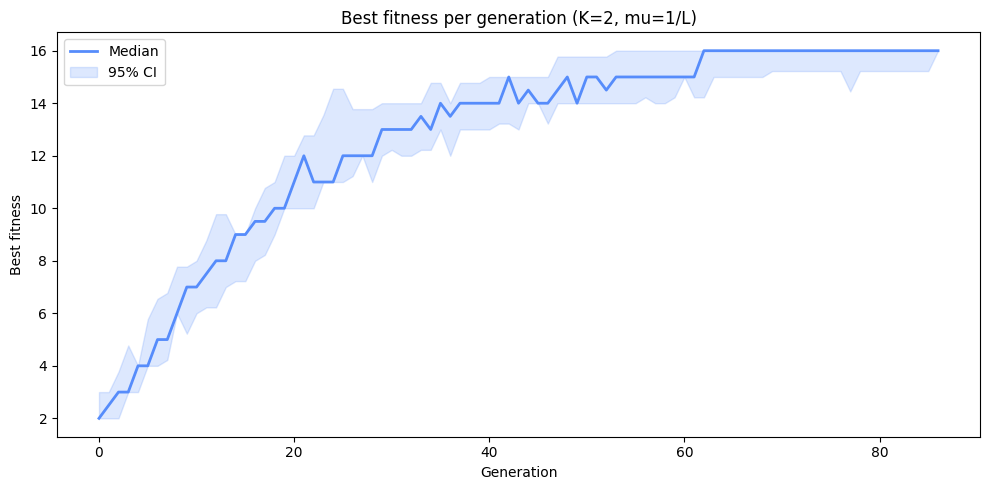
\includegraphics[width=0.7\linewidth]{b1_output1}
	\caption{Results of running the GA 10 times with baseline values ($K=2$, $\mu=1/L$, $N=200$). The blue line shoes the median over 10 samples, while the light blue shaded area shows the confidence interval.}
	\label{fig:b1output}
\end{figure}

With the baseline values, the algorithm finds the correct results within 86 generations for all 10 samples, but usually earlier \ref{fig:b1output}. The average generation count till $t_{\text{finish}}$ is 61.9.


\todo[inline]{Caption is too terse. Spell out axes, the baseline ($K=2$, $\mu=1/L$, $N=200$), what the bands/lines represent (mean best fitness with shaded $\pm$ std across 10 runs?), and the take-home (``all 10 runs find the target within $\sim\!X$ generations''). Same applies to every other figure below --- captions should be self-contained.}
\begin{figure}[H]
	\centering
	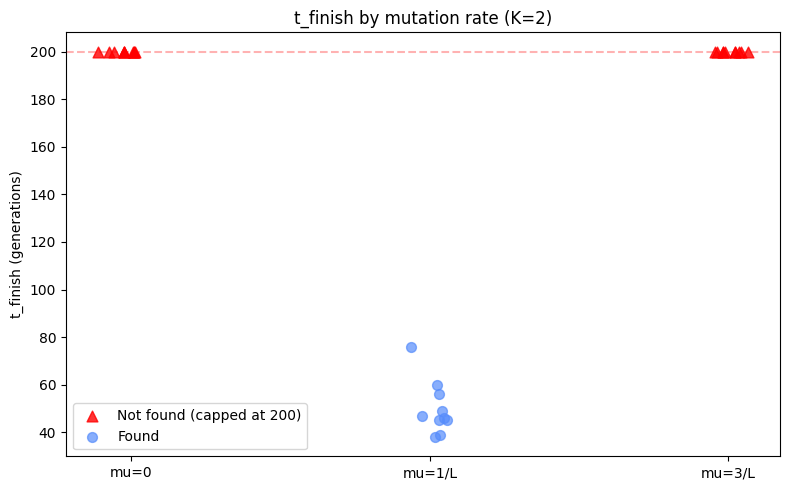
\includegraphics[width=0.7\linewidth]{b1_output2} 
	\caption{Three different mutation rates with K=2. Of these mutation rates, the GA manages to find the target only with mu=1/L before getting cut off at 200 Generations}
	\label{fig:b1output2}
\end{figure}



\begin{figure}[H]
	\centering
	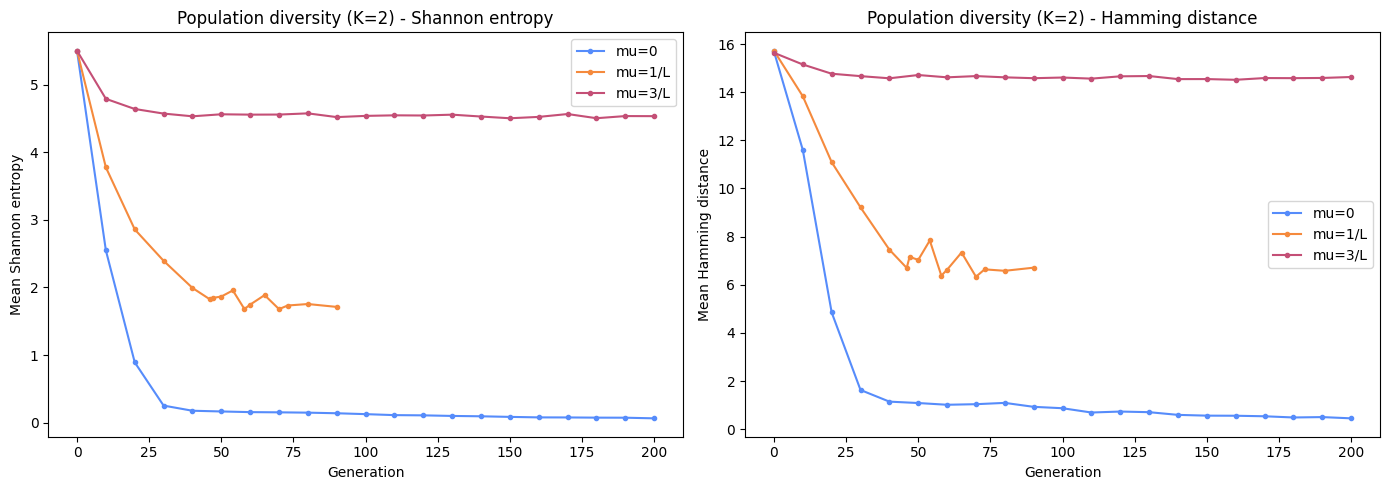
\includegraphics[width=0.7\linewidth]{b1_output3}
	\caption{Measuring the diversity of the runs in two different ways, with Shannon entropy and Hamming distance. Both show that mu=0 leads to no diversity, mu=3/L leads to high diversity through randomness while mu=1/L manages to strike a middle ground (and reach the target).}
	\label{fig:b1output3}
\todo[inline]{Fix typo ``entrophy'' $\to$ ``entropy''. Specify what ``diversity'' is on the y-axis (mean pairwise Hamming distance / mean position-wise Shannon entropy in nats or bits?). Clarify whether this is averaged over the 10 runs and whether the band is std or min/max.}
\end{figure}
\begin{figure}[H]
	\centering
	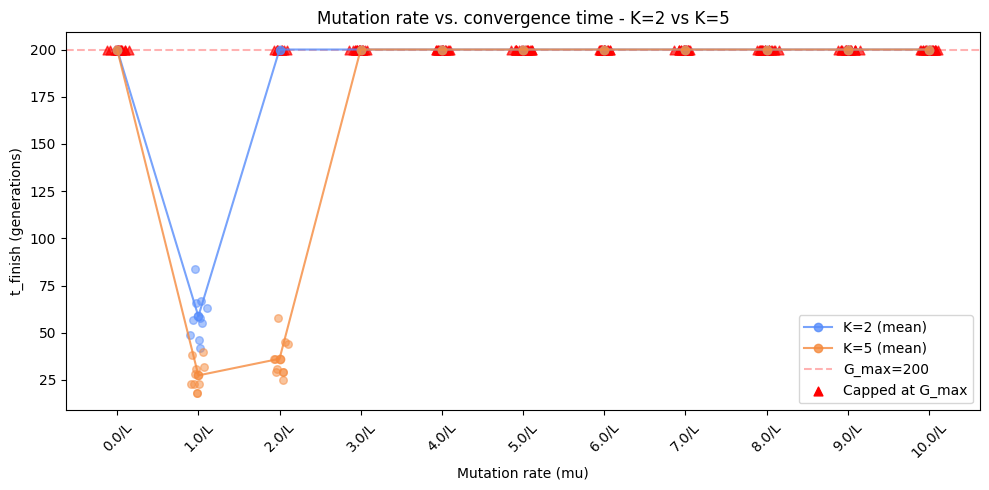
\includegraphics[width=0.7\linewidth]{b1_output4}
	\caption{Higher tournament size increases selection pressure. We repeat the mu sweep to see how this interacts with mutation rate. K=5 leads to results faster \& can also converge with mu=2/L, though mu=1/L remains optimal.}
	\label{fig:b1output4}
\end{figure}
\todo[inline]{MISSING FIGURE for B.1 Q5: a plot of $\mu$ vs $t_{\text{finish}}$ over $\sim$10 $\mu$ values from 0 to $10/L$, with the optimum annotated. The parameter table already promises this sweep --- deliver the figure and state the optimal $\mu$ in prose (e.g. ``$\mu^\star \approx 1/L$ for $K=2$, shifting toward $\approx 2/L$ for $K=5$'').}
\todo[inline]{Add a short ``B1 take-away'' paragraph after the figures: (1) optimal $\mu \approx 1/L$; (2) too low $\mu$ $\to$ premature convergence (diversity collapse visible in Fig.~\ref{fig:b1output3}); (3) too high $\mu$ $\to$ random walk, never converges; (4) higher $K$ shifts tolerable $\mu$ upward (more selection pressure compensates for more noise). This directly answers B.1 Q4 and Q6.}






\subsubsection*{B2}
\todo[inline]{Add a short intro paragraph before the figures: restate the research question (``does 2-opt local search improve TSP performance beyond the extra compute it costs?''), name the two datasets, and preview that the fair-comparison answer requires wall-clock normalisation (you already argue this below --- move the argument up so the figures land with context).}




\begin{figure}[H]
	\centering
	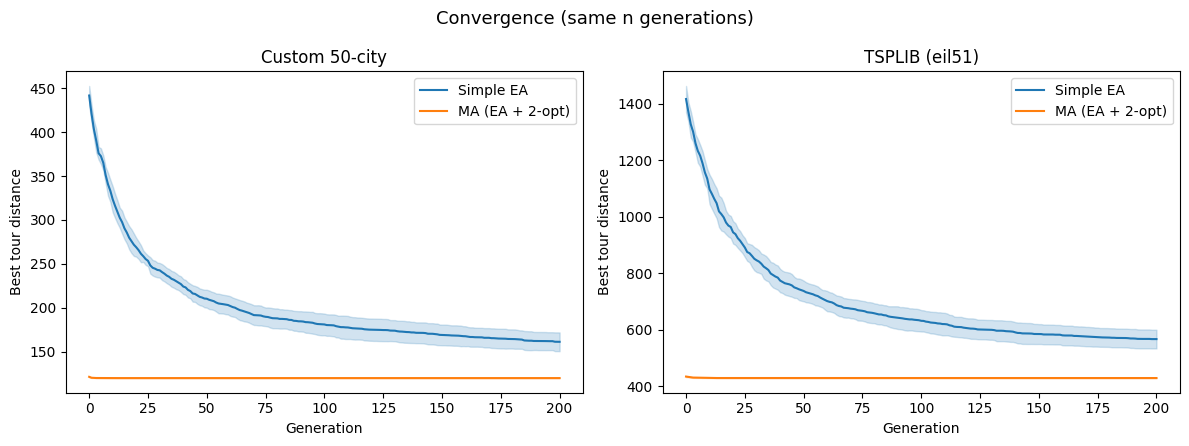
\includegraphics[width=0.7\linewidth]{b2_output1}
	\caption{Both of the datasets show MA reaching better results in fewer generations, and in total.}
	\label{fig:b2output1}
\todo[inline]{Caption should name the datasets on each panel, the y-axis (mean best tour length in same units as the coordinates?), and what the shaded band is. Also state the gap numerically (e.g. MA $\approx X$, EA $\approx Y$ on eil51; known optimum for eil51 is $426$, mention it).}
\end{figure}
\begin{figure}[H]
	\centering
	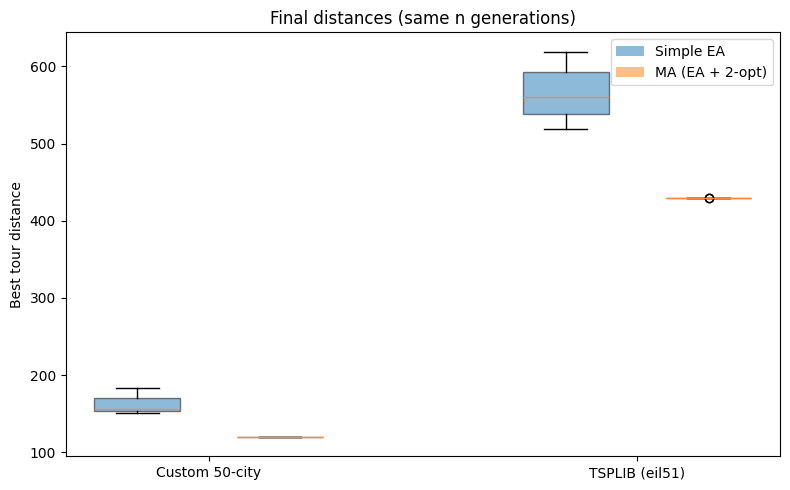
\includegraphics[width=0.7\linewidth]{b2_output2}
	\caption{In this comparison, MA clearly beats EA in distance and consistency.}
	\label{fig:b2output2}
\todo[inline]{``Consistency'' --- quantify. Report std or IQR of final tour length across 10 runs for each (dataset, algorithm). Consider a Mann--Whitney U test on final tour lengths to support the claim with a $p$-value; the rubric (``Validity'') rewards statistical backing of claims.}
\end{figure}
\begin{figure}[H]
	\centering
	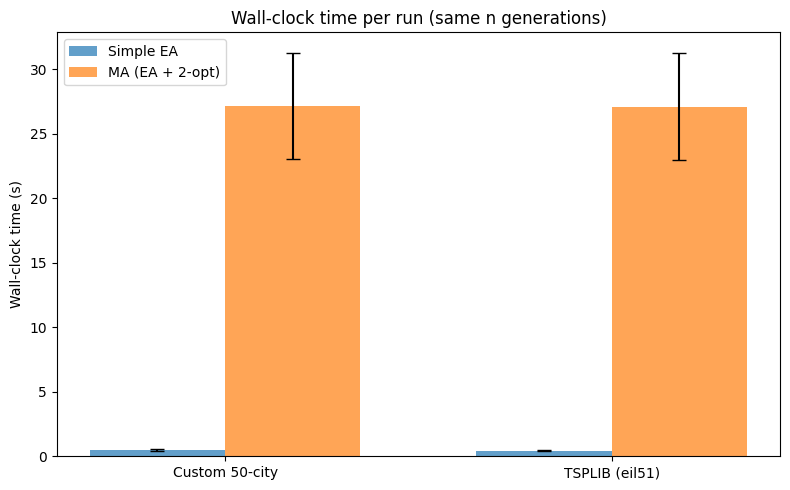
\includegraphics[width=0.7\linewidth]{b2_output3}
	\caption{Per generation, MA takes much more compute \& longer than EA. It is therefore not fair to compare them in this way.}
	\label{fig:b2output3}
\end{figure}

We considered comparing them on number of operations, but the operations of MA are only in its neighborhood, so comparing them directly with whole generations of EA would again be unfair. We therefore decided to compare wall-clock time that, while influenceable by all kinds of factors and therefore not overly scientific, provides a good baseline for real-use performance, especially if averaged over 10 runs each.

Comparing the MA and simple EA on the same number of generations is not a fair baseline. Each MA generation includes a full 2-opt local search over every individual in the population, making it far more computationally expensive than a single EA generation. Any advantage observed per generation could therefore reflect additional computation rather than algorithmic superiority. We considered normalizing by number of fitness evaluations, but since 2-opt operates within a solution's neighborhood its evaluation count is not directly comparable to a full population generation in the EA. We therefore compare on wall-clock time, which - while sensitive to system-level factors - provides a practical performance baseline when averaged over 10 runs.

\begin{figure}[H]
	\centering
	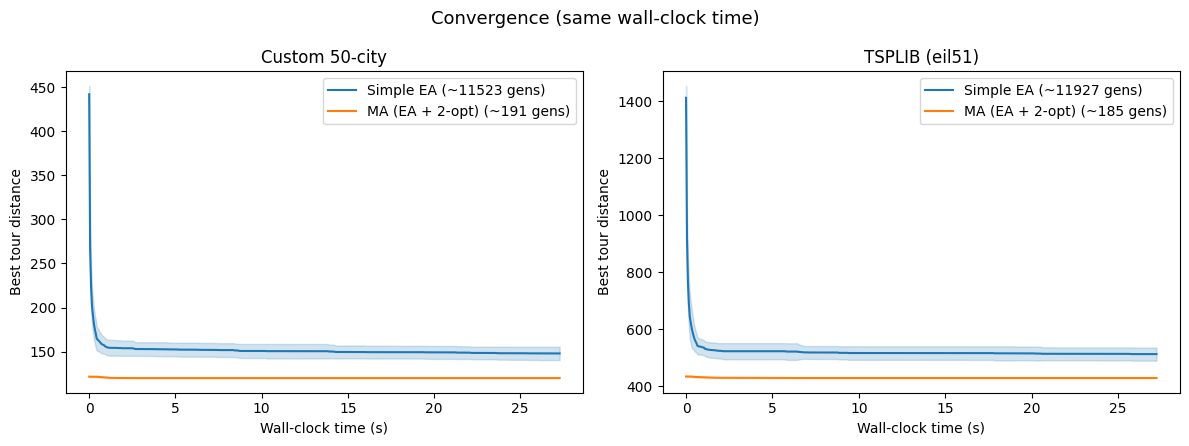
\includegraphics[width=0.7\linewidth]{b2_output4}
	\caption{If compared instead on wall-clock time, MA still converges on better values, but EA's curve also flattens to near its best result in a comparable time as MA. While EA goes through more than 11-thousand generations in this time, MA only reaches around 190.}
	\label{fig:b2output4}
\end{figure}
\begin{figure}[H]
	\centering
	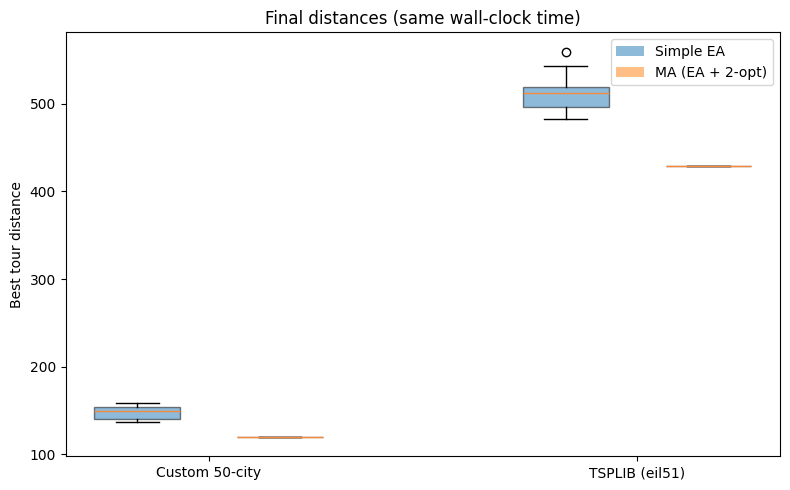
\includegraphics[width=0.7\linewidth]{b2_output5}
	\caption{While the gap has shrunk considerably from comparing by number of generations, MA still provides better and more consistent results than EA.}
	\label{fig:b2output5}
\end{figure}

Even under a fair wall-clock comparison, the MA consistently reaches shorter and more consistent tour distances than the simple EA on both datasets. The addition of local search therefore genuinely improves performance beyond what the extra computation alone can explain: 2-opt allows individuals to escape local optima that trap the plain EA, reducing both mean tour length and variance across runs.
\todo[inline]{This is the core conclusion of B.2 --- strengthen it with numbers: ``On eil51, MA reached mean tour length $X \pm s_X$ vs EA's $Y \pm s_Y$ within the same wall-clock budget of $T$\,s (Mann--Whitney $U$, $p < 0.01$).'' Without numbers this reads as an assertion.}
\todo[inline]{Note the two paragraphs above (the ``We considered\ldots'' block and the ``Comparing the MA\ldots'' block) are near-duplicates of each other --- one is clearly an earlier draft. Keep the better one (the second is more polished) and delete the other.}


\subsection*{Discussion}

Several limitations of this study should be noted. All experiments were run on a single machine, and the results may differ on other 
hardware or with a more optimised 2-opt implementation, which are all factors which may affect the wall-clock time. With only 10 runs 
per condition the confidence intervals are modest, particularly at boundary mutation rates where success is inconsistent, and formal statistical tests (e.g.\ Wilcoxon rank-sum) would be needed to make stronger claims. 
Only two TSP instances were tested and only one target string was used for the string search task, so the generalisability of the findings is 
limited. Regarding threats to validity, 2-opt is a heuristic specifically tailored to tour optimisation problems, so the advantage of the 
MA over the plain EA may not transfer to other combinatorial problems where no efficient local search is available. Additionally, censoring 
$t_{\text{finish}}$ at $G_{\max} = 200$ when the target is not found biases mean convergence time downward, meaning the true performance gap 
between mutation rates is likely larger than reported. Future work could test the MA on larger TSPLIB instances to assess scalability, vary 
the intensity of local search (e.g.\ full 2-opt vs.\ a fixed number of improvement steps, or Baldwinian rather than Lamarckian learning), 
and explore adaptive mutation rates that adjust $\mu$ dynamically as population diversity changes.

% \todo[inline]{EMPTY. Add 4--6 sentences. Must cover: (1) limitations --- wall-clock is hardware/implementation-dependent, single machine, 10 runs is modest, only two TSP instances tested, only one target string; (2) threats to validity --- 2-opt is specialized to TSP so the MA advantage may not generalize; censoring of $t_{\text{finish}}$ at $G_{\max}$ biases the mean downward; (3) future work --- test on larger TSPLIB instances, vary 2-opt intensity (full vs. $k$ steps, Baldwinian vs Lamarckian), try adaptive $\mu$. The rubric explicitly mentions ``discuss some potential limitations''.}


\subsection*{Conclusion}
This project shows that small changes in EA design choices have large and predictable effects on performance. For string search, the mutation 
rate $\mu = 1/L$ is optimal as it provides enough exploration to maintain diversity and avoid premature convergence, without being so disruptive 
that accumulated progress is lost. Increasing tournament size to $K = 5$ raises selection pressure, accelerating convergence and shifting the 
viable mutation range upward, though the optimum remains $\mu = 1/L$. For the TSP, the memetic algorithm consistently outperforms the plain EA 
in both solution quality and consistency, and this advantage holds even under a fair wall-clock comparison that accounts for the roughly 25 times
higher cost per MA generation. Furthermore, 2-opt local search allows individuals to escape the local optima that cause high variability in the plain EA. 
The take-home message is that local search is worth its computational cost for TSP, while for string search there is a narrow optimal mutation 
rate whose precise value shifts with selection pressure. Both findings reflect the same underlying principle that effective evolutionary search 
requires a carefully tuned balance between exploration and exploitation.
% \todo[inline]{EMPTY. The rubric (``Clarity'' + assignment ``take-home message'') makes this section worth real points. Write 4--6 sentences covering: (1) the main finding on B1 --- optimal $\mu \approx 1/L$ balances exploration and exploitation, and higher $K$ shifts this upward; (2) the main finding on B2 --- MA beats EA even under a fair wall-clock comparison because 2-opt escapes local optima; (3) one-sentence take-home: ``local search is worth its compute cost for TSP; for string search there is a narrow optimal mutation rate that depends on selection pressure.''}



\newpage
\appendix
\section*{Appendix}
\subsection*{Part A}
\subsection*{A1}
What can you conclude about the effects of fitness scaling on selection pressure?

Adding constants raises all fitness all values by that amount. So it smooths out all the values. For example, when we compare f2 (which only squares X) and f4 (which squares X and adds 20), we can see that the probabilities of f4 are closer together. Probabilities are increased and reduced, so there is a much smaller gap between them, which also reduces selection pressure. 
Multiplying by a constant does not change the selection probabilities. If we compare f2 and f3, we can see that the probabilities stay the same even if we scale it. So scaling fitness does not have an effect on the selection pressure.



\begin{figure}[H]
	\centering
	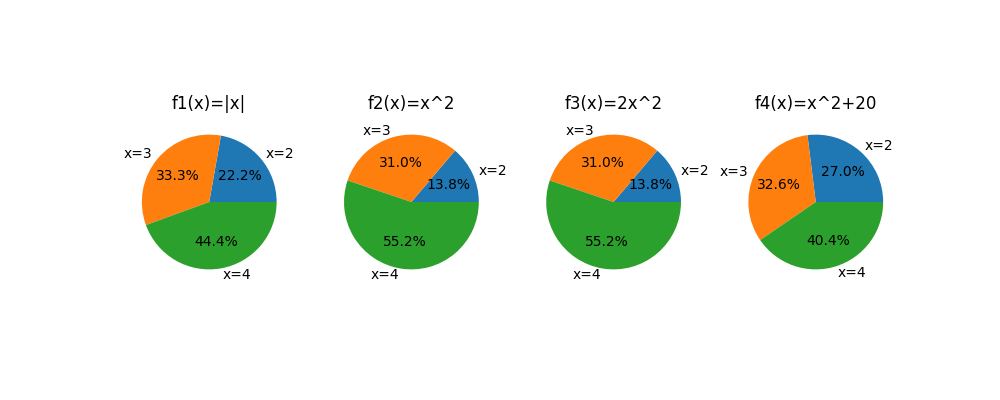
\includegraphics[width=0.7\linewidth]{pie_charts}
	\caption{Selection probability of the three individuals for each
function.}
	\label{fig:pie_charts}
\end{figure}



\begin{table}[h]
\centering
\begin{tabular}{c c c c c c c c c}
\hline
x & f1 & p1 & f2 & p2 & f3 & p3 & f4 & p4 \\
\hline
2 & 2 & 0.2222 & 4  & 0.1379 & 8  & 0.1379 & 24 & 0.2697 \\
3 & 3 & 0.3333 & 9  & 0.3103 & 18 & 0.3103 & 29 & 0.3258 \\
4 & 4 & 0.4444 & 16 & 0.5517 & 32 & 0.5517 & 36 & 0.4045 \\
\hline
\end{tabular}
\caption{Fitness function value and selection probability for each individual and each
function.}
\end{table}


\subsection*{A2}

Does the algorithm find the optimum?
Yes. It is able to reach fitness 100, meaning all 100 bits were successfully set to 1. 

What do you see?
The version without selection is stuck at around 50 and never converges. The version with selection keeps steadily climbing, ultimately reaching 100.

Can you conclude anything on the difference between these two versions based on the above results? If yes, why? If not, what should you do to make a fair comparison? 
No. We would need multiple runs as EAs are stochastic and each run produces different results because of initialization and random mutation. To make it fair, we should run each version multiple times and use averages. 

Is there a difference in performance?
Yes. It is apparent that there is a difference in performance between the versions. Across all the runs, the version with selection always converges to fitness 100 while the version without selection is always near 50 through all the 1500 generations. The algorithm has no memory of good solutions and cannot improve. 


\begin{figure}[H]
    \centering
    \begin{minipage}{0.48\linewidth}
        \centering
        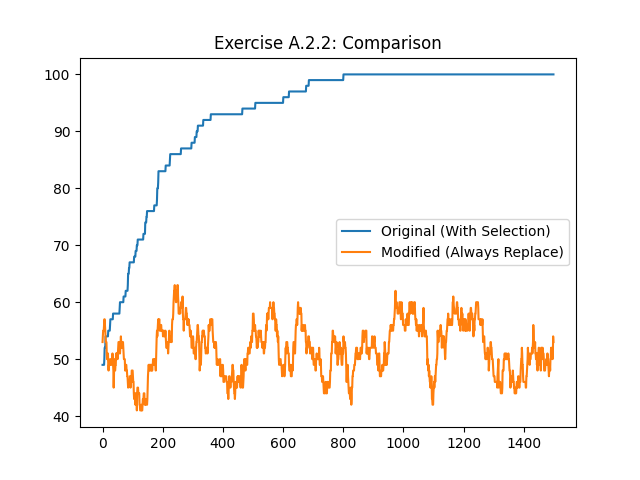
\includegraphics[width=\linewidth]{fitness_vs_generations}
        \caption{Fitness against generations.}
        \label{fig:fitness_vs_generations}
    \end{minipage}
    \hfill
    \begin{minipage}{0.48\linewidth}
        \centering
        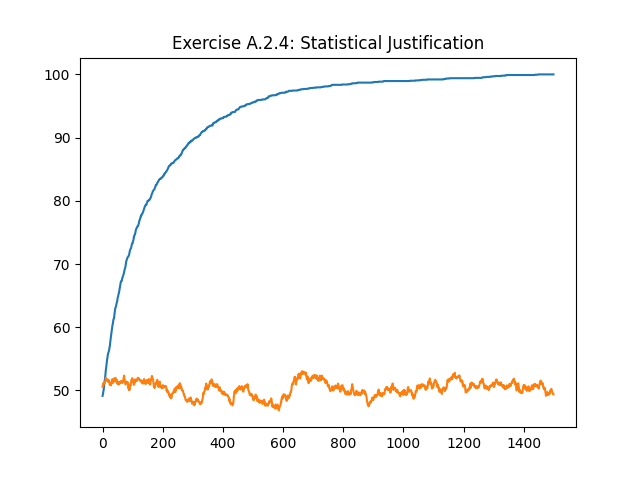
\includegraphics[width=\linewidth]{fitness_vs_generations_avg}
        \caption{Averages of fitness vs generations across multiple runs.}
        \label{fig:fitness_vs_generations_avg}
    \end{minipage}
\end{figure}
\end{document}